% 3rd - Recognition
%% Includes: Alignment methods, matching, descriptors, hypothesis verification

\chapter{Sparse feature matching}
\label{cha:feature}

Solutions to problem stated in section \ref{sec:problem} are commonly divided \cite{something} into feature-based and template-based. The former approach, also referred to as local matching, is focused on comparing point neighbourhoods between the scene and model datasets. 

The solution in such methods is composed of several steps. Firstly, an input subset with elements of rich and distinguishable neighbourhood information is selected. Points that belong to this subset are referred to as \textit{keypoints}. For each keypoint, its neighbourhood information is expressed in the form of a \textit{descriptor} vector. By the means of selected metric, commonly the $L_2$ norm, descriptors are further compared between the scene and model datasets, to find \textit{correspondences} with minimal distance. Such point pairs are then grouped to share similar geometric constrains and finally, the largest clusters are used to calculate affine transformation, which renders the initial problem solution.

The inherent locality of feature matching methods has direct implications on the solution performance. Such methods are by design robust to occlusions \cite{something}. Each point is processed independently, which enables data parallelization to boost time performance. Conversely, keypoint identification requires costly analysis of the whole input dataset, thus a balance between the recognition performance and time effectiveness is required \cite{somethin} for real-time applications.

%---------------------------------------------------------------------------

\section{Shape description} %SHOT}
\label{sec:shape} %shot}

There is a multitude of proposals for shape key-point detectors existing in literature. An overview and performance evaluation of the most popular methods can be found in \cite{keypoints1} and \cite{keypoints2}. From both evaluations, the \textit{Intrinsic Shape Signatures} (ISS) \cite{ISS} detecor is worth particular attention. \cite{keypoints1} states that ISS, as a fixed-scale detector, copes well with full three-dimensional models and provides a proper balance between the repeatability rate and time efficiency. In \cite{keypoints2}, the ISS is evaluated with the best repeatability rate among detector implementations available in PCL. The ISS introduces a saliency measure, defined by the smallest eigenvalue of the neighbourhood scatter matrix. For a given point $p$ and its neighbourhood $N$, the scatter matrix $\Sigma$ is given by
\begin{equation}
\label{eq:scatter}
\Sigma(p,N) = \frac{1}{|N|} \sum\limits_{q\in N}(q -\mu_p)(q - \mu_p)^T,\ \mu_p = \frac{1}{|N|}\sum\limits_{q\in N}q
\end{equation}
% originally defined as weighted matrix, need to check how its implemented
By denoting the eigenvalues of $\Sigma(p, N)$ as $\lambda_1 > \lambda_2 > \lambda_3$, the ISS detector classifies $p$ as a keypoint, if the following condition is satisfied
\begin{equation}
\label{iss}
\frac{\lambda_2}{\lambda_1} < \epsilon_1 \  \land \  \frac{\lambda_3}{\lambda_2} < \epsilon_2 \ \land \  \lambda_3 > \epsilon_3.
\end{equation} 
Thresholds $\epsilon_1$ and $\epsilon_2$ are meant to provide sufficient difference between variations along each principal direction, which aids in estimation of a repeatable reference frames for further description stages. The third threshold $\epsilon_3$ ensures that the variations are large enough to consider the point as interesting. A further improvement to the ISS detection criteria is to apply non-maximum suppression over the saliency measure computed at each point. With this edge thinning technique, a point is classified as a keypoint, if it has the largest $l_3$ over its neighbourhood.  An example of keypoints detected with ISS is presented on figure \ref{fig:iss}. The object (cleaning spray in the center of the figure) has marked points in areas of rich shape information, like the bottleneck or the nozzle. It is also visible, that ISS classifies wrong points in two cases. Firstly, when a point lies on a visibility boundary (i.e. the edges of flat surfaces in the figure), thus it should be extended with boundary detection as described in xx. Secondly, when the sensor noise is high (distant wall flat surface in upper left edge of the figure). This issue can be handled by ignoring points above certain z-distance from the sensor or by adaptatively selecting neighbourhood radius for saliency measure.
%select rich shape object from willow = 13
%implement hardload and iss, measure avg time
%implement in cuda

\begin{figure}[h]
\centering
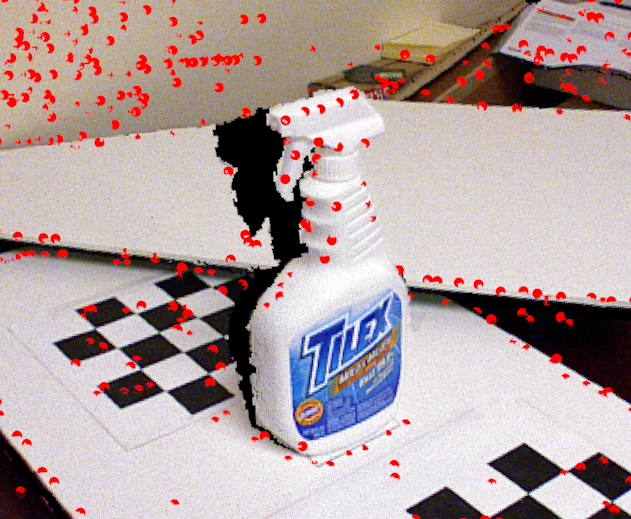
\includegraphics[width=0.8\textwidth]{fig/ISS}
\caption{ISS keypoints (marked with red) computed with $\epsilon_1 =  \epsilon_2 = 0.75$ and $\epsilon_3 = 0.0005$ }
\label{fig:iss}
\end{figure}

The overall time complexity of ISS classification is at the order of $O(nk)$, where $n$ is the image size and $k$ is the max neighbourhood size. This translates into average execution times on target platforms, provided in table \ref{tab:issexec}.

\textit{the ISS method with boundary point re-
moval (ISS-BR) was used to detect the keypoints in the
scene and the models. As reported in (Salti et al, 2012),
ISS achieves the best performance compared to other
keypoint detectors when used in conjunction with fea-
ture descriptors.}

\begin{table}[h]
\centering
\begin{tabular}{r || c | c}
& NVidia Jetson TK1 & Lenovo Y50-70 \\
 \hline
 \hline
 PCL ISS& 4s & 4s \\
 PCL ISSBD& 4s &  4s \\
 CUDA ISS& 4s & 4s \\
 CUDA ISSBD& 4s & 4s
\end{tabular}
\caption{ISS detector time performance statistics.}
\label{tab:issexec}
\end{table}

It is important to note, that in practical applications the keypoint detection step is often replaced by volumetric down sampling. About voxel grid. Model is densely grained. This avoids computational costs of keypoint detection, but increases the complexity of further matching and clustering stages. How to choose this tradeoff.
%In \cite{keypoints-learning}, authors propose a random-forest classifier to be trained for detection of the best interest points for any chosen descriptor.

%Provide complexity, measure time perf (and invariance to transformations?). Can be skipped with uniform.

%A descriptor is considered to be reliable if it is able to capture the same surface characteristics, regardless of rigid transformations, varying sampling density and noise.

Similarly to keypoint detection methods, the literature also abounds with different keypoint description proposals. A comprehensive comparison of the most common methods can be found in \cite{descriptorsComparison}. The \textit{Fast Point Feature Histograms} (FPFH) \cite{FPFH, FPFH2} and \textit{Signature of Histograms of OrienTations} (SHOT) \cite{SHOT} descriptors are particularly interesting for the purposes of this work, given the real-time execution assumptions.


FPFH represents the relative orientation of normal vectors between the query point $p$ and each of its neighbours $q \in N$. For each point pair $(p, q)$, a new coordinate frame $u,v,w$ originating at $p$ is constructed as
\begin{equation}
u = n,\  v = n \times \frac{p-q}{\|p-q\|_2},\  w = u \times v,
\end{equation}
where $n$ is the normal vector at $p$ and $d = \|p-q\|_2$ is the Euclidean distance. Using this reference frame, the difference between normals at $p$ and $q$ is expressed by the angular features
\begin{equation}
\alpha = v \cdot n, \  \phi = u \cdot \frac{(p-q)}{\|p-q\|_2}, \ \theta = \arctan(w\cdot n, u \cdot n).
\label{eq:fpfhangulars}
\end{equation}
The angular features are further binned into a histogram $H$, typically dividing them into $5$ subdivisions, which leads to $3^5=125$ bins. WRONG! FPFHs are decorrelated, 11binned = 33bins. Such histograms are computed every point in the input point cloud. Finally, the FPFH descriptor is formed as
\begin{equation}
FPFH(p) = H(p) + \frac{1}{|N(p)|}\sum\limits_{q\in N(p)}\frac{1}{ \|p-q\|_2}H(q).
\end{equation}
The FPFH descriptor computational complexity is $O(nk)$.


The SHOT proposal emphasises the importance of defining a unique and unambiguous local coordinate system, namely the \textit{Local Reference Frame} (LRF), as a basis for a comparable descriptor construction. A modified version of support covariance matrix (as defined in eq. \ref{eq:scatter}) is introduced, where each neighbour is weighted by its proximity to the query point: 
\begin{equation}
\label{eq:weighCov}
M(p) = \frac{1}{\sum\limits_{q\in N(p)}(r - \|p-q\|_2)} \sum\limits_{q\in N(p)}(r - \|p-q\|_2)(p - q)(p - q)^T.
\end{equation}
The authors determine the LRF coordinate system axes, $x$, $y$ and $z$ with the corresponding eigenvectors of $M$, $e_x$, $e_y$ and $e_z$ in decreasing eigenvalue order. The sign of the axes is disambiguated by aligning the orientation of $x$ and $z$ axes with the majority of vectors they are representing. Concretely, the signed $x$ axis is given by the formula
\begin{equation}
x(p) = \begin{cases}\ e_x, & \mbox{if } \sum\limits_{q \in N(p)} \operatorname{sign}\left( (p-q)^T \cdot x \right) \geq 0 \\ -e_x, & \mbox{otherwise} \end{cases}.
\end{equation}
The $z$ axis sign is determined analogically and $y$ is a cross product of the former, $y = z \times x$. The authors have proven experimentally a high repeatability of such LRF, even in presence of noise and clutter. To form a descriptor, support is further divided with a spherical grid of 2 radial, 2 elevation and 8 azimuth divisions, as depicted on figure \ref{fig:shotgrid} (for better visibility, only half of azmiuth partitions are shown), resulting in 32 cells total.  For each cell, the cosine of the angles $\theta_q$ between the normal at the query point $n_p$ and each normal at cell points $n_q$ are binned to form a histogram. Uniform binning of the cosine function provides robustness to LRF perturbations, as it leads to coarser angle binning for normals close to the $z$ axis. Another problem, called \textit{boundary effect}, arises due to the rough division of the support volume. Depending on the inaccuracies in LRF estimation, points that are close to the boundaries between neighbouring cells are not repeatably accounted to the same histogram. To avoid this problem, the authors propose to interpolate the neighbouring bins to spread the counts among them. After this step, the local histograms are being normalized by their $L_2$ norms, to account for varying point densities. Finally, the SHOT descriptor is composed by concatenating the local histograms, each with typically of 11 bins, resulting in 352 element descriptor.

\usetikzlibrary{3d}

\begin{figure}[h]
\centering
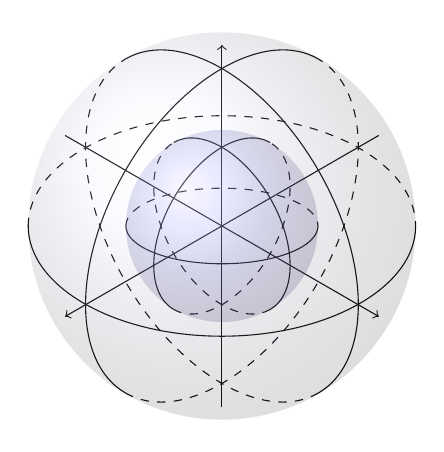
\begin{tikzpicture}[scale=2]
   \begin{scope}[x={(330:1cm)},y={(210:1cm)},z={(90:1cm)}]
    \begin{scope}[canvas is zy plane at x=0]
     \draw (135:1cm) arc (135:-45:1cm);
     \draw[dashed] (135:1cm) arc (135:315:1cm);  
     \draw (135:0.5cm) arc (135:-45:0.5cm);
     \draw[dashed] (135:0.5cm) arc (135:315:0.5cm);   
    \end{scope}
    \begin{scope}[canvas is zx plane at y=0]
     \draw (135:1cm) arc (135:-45:1cm);
     \draw[dashed] (135:1cm) arc (135:315:1cm);
     \draw (135:0.5cm) arc (135:-45:0.5cm);
     \draw[dashed] (135:0.5cm) arc (135:315:0.5cm);   
    \end{scope}
    \draw[->] (0,0,-1.15) -- (0,0,1.15);
    \draw[->] (0,-1.15,0) -- (0,1.15,0);
    \draw[->] (-1.15,0,0) -- (1.15,0,0);
   \end{scope};
   \draw (-1.23,0) arc (180:360:1.23cm and 0.7cm);
   \draw[dashed] (-1.23,0) arc (180:0:1.23cm and 0.7cm);
   \draw (-0.61,0) arc (180:360:0.61cm and 0.24cm);
   \draw[dashed] (-0.61,0) arc (180:0:0.61cm and 0.24cm);

   \shade[ball color=blue!10!white,opacity=0.20] (0,0) circle (1.23cm);
   \shade[ball color=blue!50!white,opacity=0.20] (0,0) circle (0.61cm);
\end{tikzpicture}
\caption{SHOT descriptor spherical grid}
\label{fig:shotgrid}
\end{figure}

%Signatures vs histograms. About SHOT. Complexity, time perf.
Extension with color. \cite{CSHOT}. Performance extension in binarized form \cite{BSHOT}.

%----------------------------	-----------------------------------------------

\section{Texture description} %ORB}
\label{sec:colour} %orb}

%TODO
% - add model2views conversion to ros_recognizer
% - test SIFT, SURF and ORB with different RGB2GREY, opponent color
% - 

In addition to the spatial information contained in RGB-D images, an important and discriminative function is also performed by the description of texture. Although there are descriptor proposals in literature that combine both information cues, the best performance is achieved when color is analysed independently of shape. This benefits in further matching phase, where descriptors of smaller sizes can be compared in the same information domain and there are overall more keypoints for grouping and generating pose hypotheses.

As compared to shape, the texture descriptors are more broadly studied and developed field. A common technique shared among these methods is the \textit{scale pyramid}.

image of the scale pyramid

SIFT, successful, most widely used \cite{SIFT}.

SURF, proposed for more efficiency \cite{SURF}.

\textit{Oriented FAST and Rotated BRIEF} (ORB) \cite{ORB} is a particularly interesting proposal, because of its real-time capabilities. As the name suggests, it is an enhancement to a two former concepts, the\textit{ Features from Accelerated Segment Test} (FAST) \cite{FAST} keypoint detector and the \textit{Binary Robust Independent
Elementary Features} (BRIEF) \cite{BRIEF} descriptor.

AKAZE \cite{AKAZE}.

All designed for grey images, RGB2GREY \cite{RGB2GREY}.

Color spaces and opponent color \cite{ColorComparison}.

Color attributes \cite{ColorAttributes}

%---------------------------------------------------------------------------

\section{Clustering}
\label{sec:clustering}

Matching.
brute force, geometric consistency, hough

%---------------------------------------------------------------------------

\section{Alignment}
\label{sec:alignment}



umeyama \cite{umeyama}, ransac

